% !Mode:: "TeX:UTF-8"

\chapter{基于卫星资料的初生对流像素级检测算法设计}[Example]


\section{基于卫星资料的初生对流数据集构建}[Number]

初生对流(CI)的物理定义为强对流天气发生前,大气各种物理量处于某种特殊的状态,换句话说初生对流的未来发展趋势应该是强对流。基于卫星资料的初生对流的标注工作,主要采用带有多通道时序的阈值法,通过当前时刻与未来15分钟和30分钟(即两帧图像)的卫星红外1(10.8um,IR1)、红外2(12um,IR2)与水汽(6.25um,WV)三个通道的信息,来标注初生对流的位置。其中共有8个阈值,其中F1到F8的分别为用以上信息设置的阈值限定指标,其中的物理意义代表了不同尺度下的云顶高度、云顶高度变化以及积云形态。其中满足任意7个阈值的像元,将会被标注为初生对流。

其中标注的阈值如下表~\ref{tb_threshold}~所示。

\begin{table}[h]
	\centering
	\label{tb_threshold}
	\caption{初生对流阈值指标}
	\begin{tabular}{c c c}
		\hline 序号 & CI预报指标 & 预报指标的判断阈值 \\
		\hline F1 & IR1亮温差 &	<0℃ \\
		 F2 &WV 与 IR1 亮温差 &	−35℃~−10℃ \\
		 F3 &IR2 与 IR1 亮温差 &	−25℃~−5℃\\
		 F4 &IR1 亮温变化率 &	<-4℃/(15 min) \\
		 F5 & IR1 亮温变化率&	∆T/(30 min)<∆T/(15 min) \\
		 F6 & IR1 亮温降低至 0℃的时间 &	<30 min \\
	 	 F7 &WV 与 IR1 亮温差变化率 &>3℃/(15 min) \\
		 F8 & IR2 与 IR1 亮温差变化率 &>2℃/(15 min) \\
		\hline 
	\end{tabular}
\end{table}

通过此多通道时序的阈值法,构造了2018年FY-4a卫星全国范围内的初生对流数据集,选取了其中对流出现较为频繁的6-10月的华南地区作为此项课题的数据集。数据集的输入数据为当前时刻t的卫星数据以及当前时刻前3帧的卫星数据序列,即t-15,t-30,t-45。数据集的输出数据为当前时刻t为基准标注的初生对流掩码图像。其中t时刻的初生对流掩码是利用上述多通道阈值法通过t时刻,t+15时刻,以及t+30时刻标注出来的。
以2018年7月15日为例,数据集一条数据可视化的效果如~\ref{tb_vis_dataset}~所示。

\begin{table}[h]
	\centering
	\label{tb_vis_dataset}
	\caption{多通道云图序列数据展示图}
	\begin{tabular}{c c c c c}
		\hline  通道 & t-45 & t-30 & t-15 & t \\
		\hline \\
		水汽通道WV &
		\begin{minipage}[b]{0.15\columnwidth}
			\centering
			\raisebox{-.5\height}{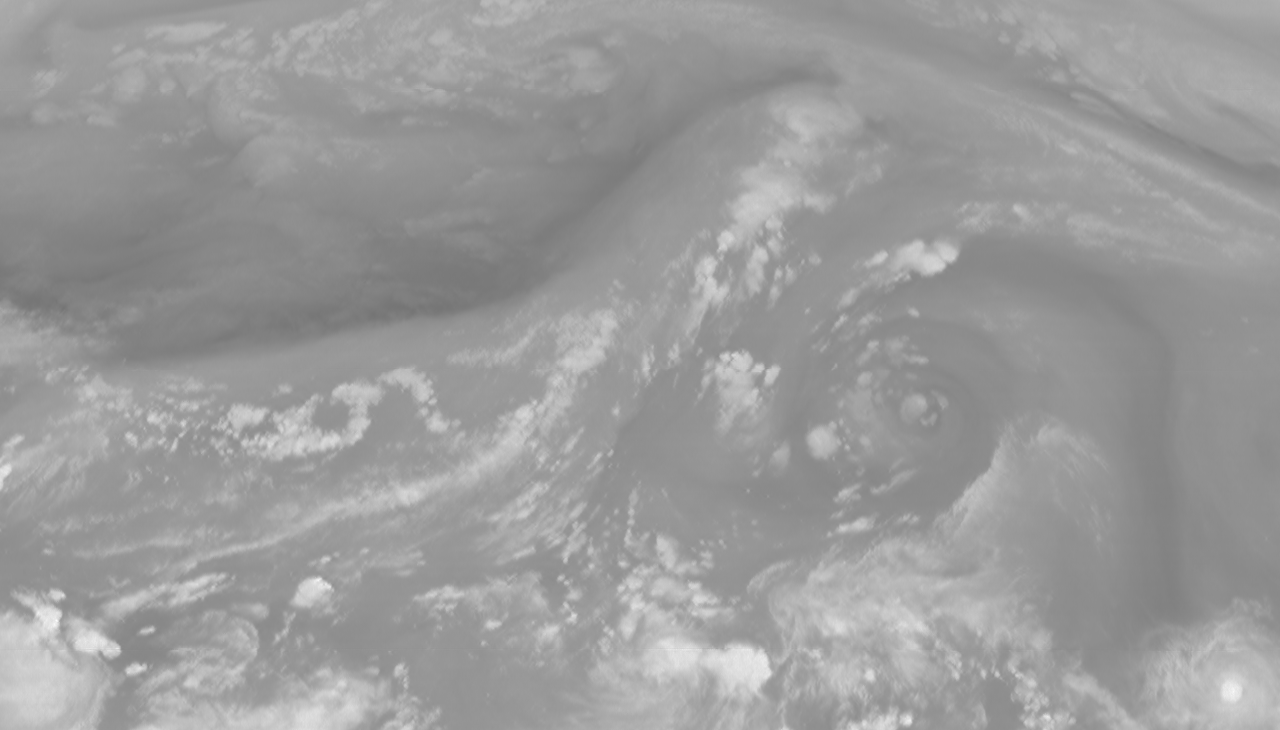
\includegraphics[width=\linewidth]{0000.png}}
		\end{minipage}&
		 \begin{minipage}[b]{0.15\columnwidth}
				 	\centering
				 	\raisebox{-.5\height}{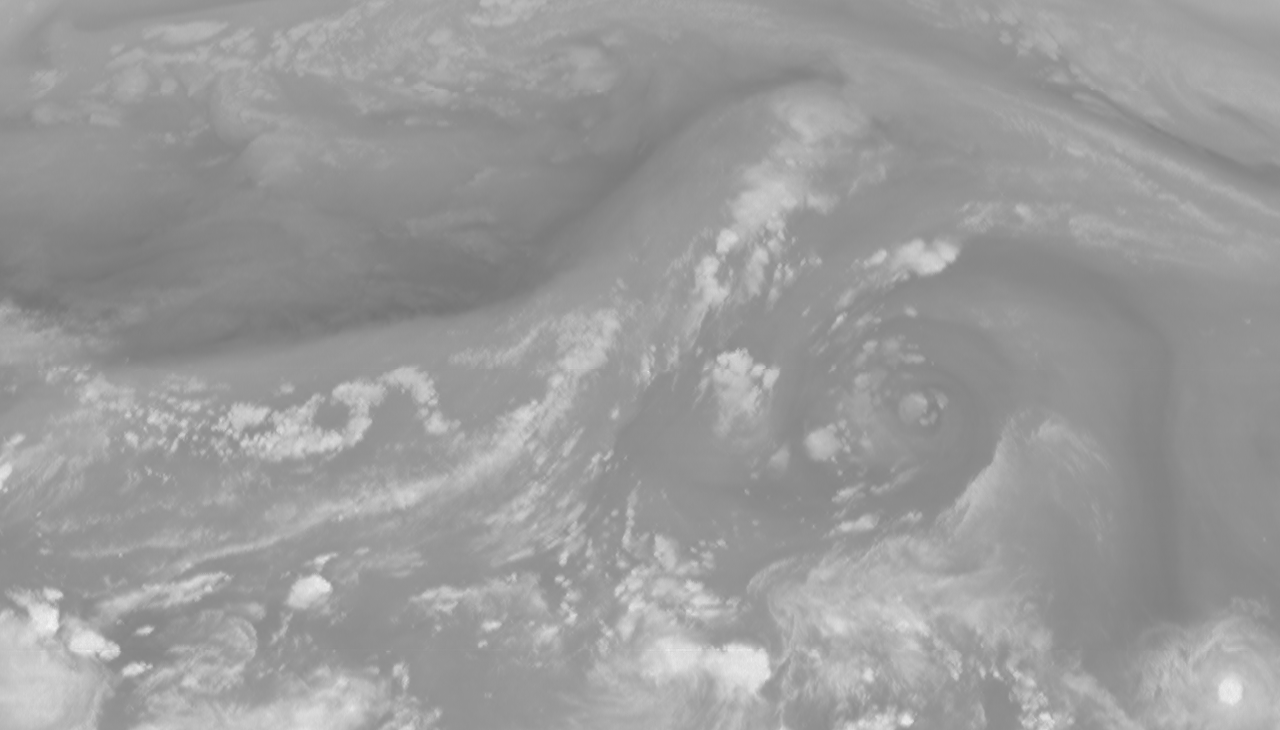
\includegraphics[width=\linewidth]{0000 (1).png}}
		 \end{minipage}&
		\begin{minipage}[b]{0.15\columnwidth}
		  	\centering
		  	\raisebox{-.5\height}{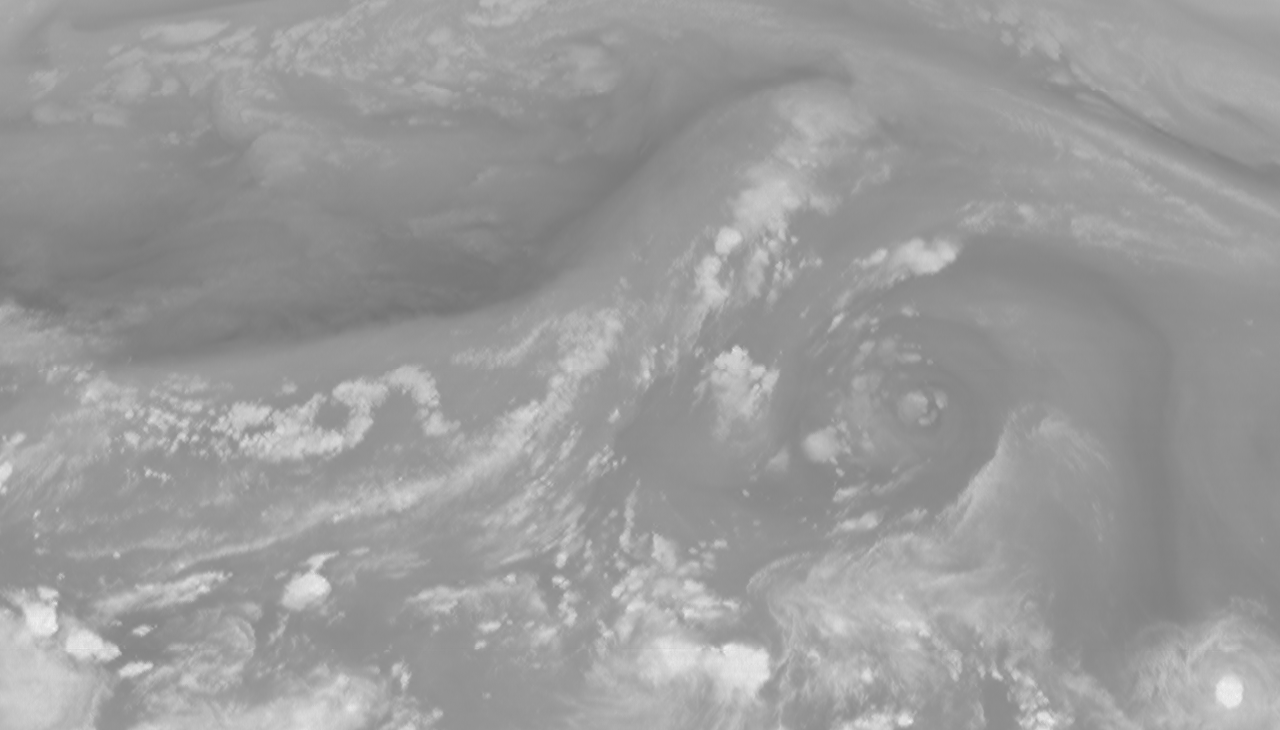
\includegraphics[width=\linewidth]{0000 (2).png}}
		\end{minipage}& 
		\begin{minipage}[b]{0.15\columnwidth}
		  	\centering
		  	\raisebox{-.5\height}{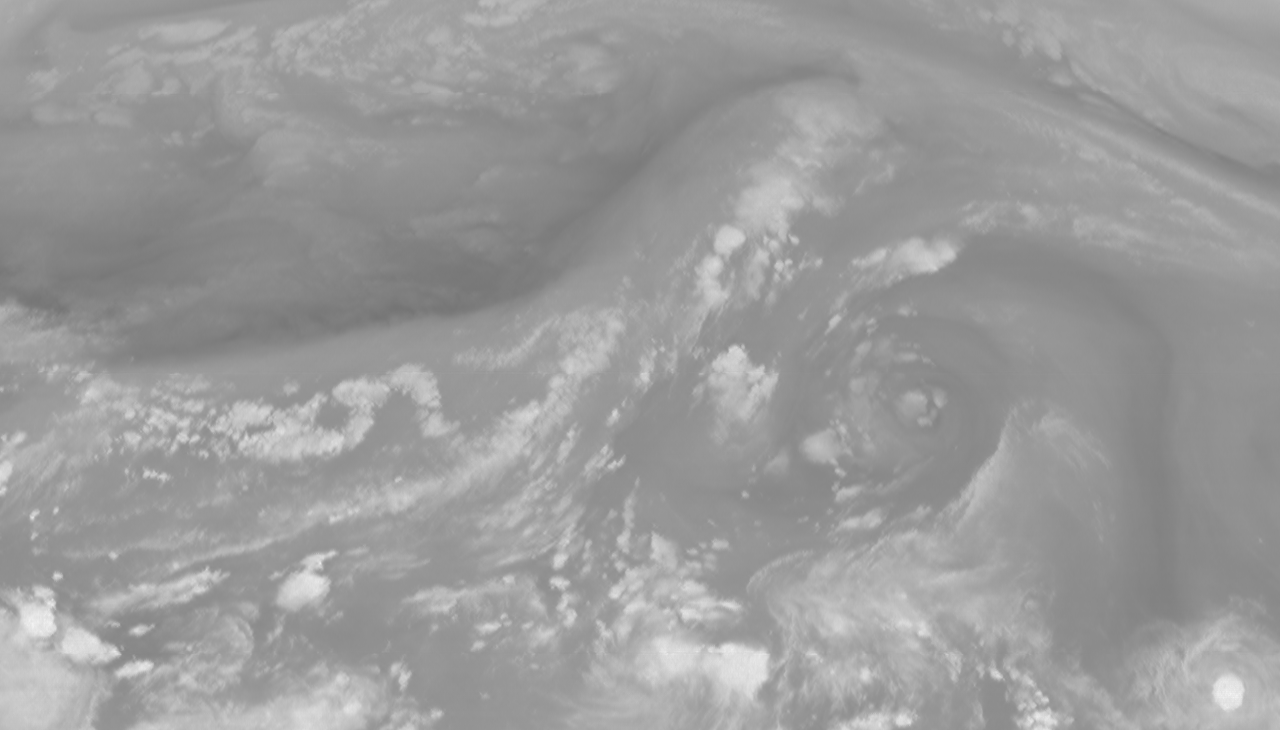
\includegraphics[width=\linewidth]{0000 (3).png}}
		\end{minipage}\\
	\\
			红外通道IR1 &
	\begin{minipage}[b]{0.15\columnwidth}
		\centering
		\raisebox{-.5\height}{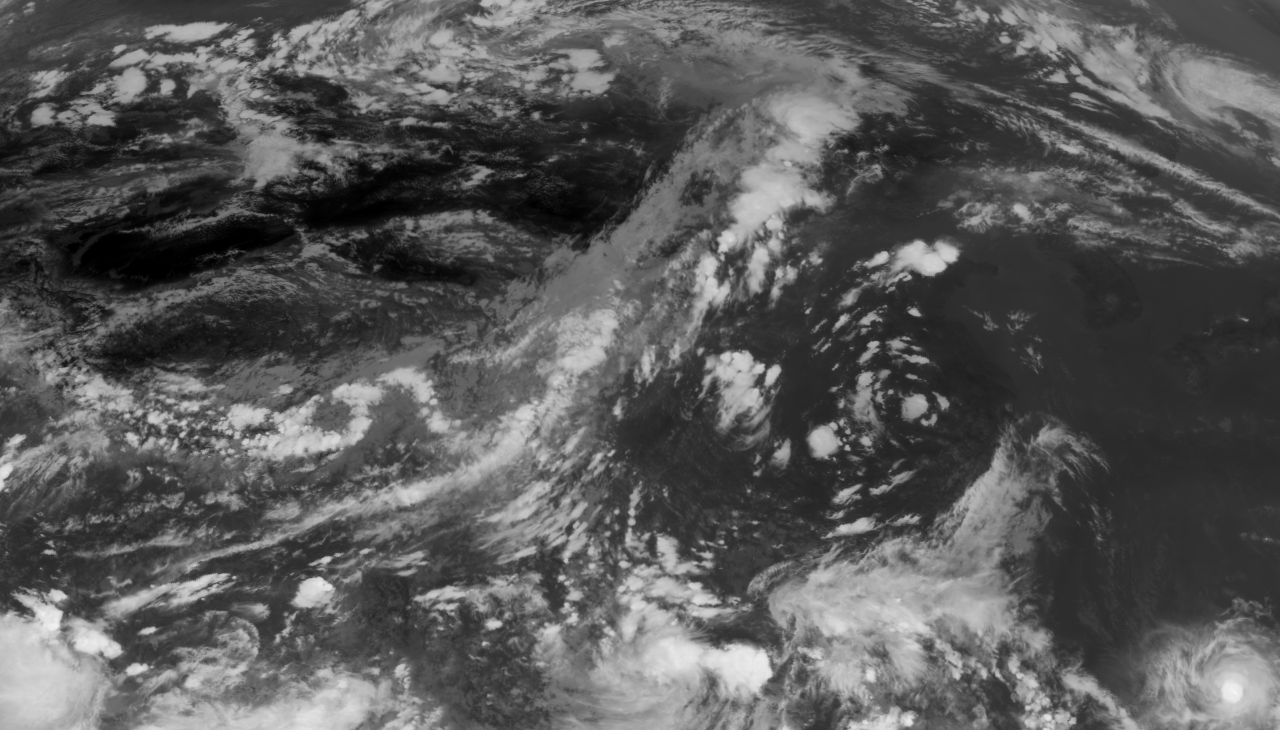
\includegraphics[width=\linewidth]{0001.png}}
	\end{minipage}&
	\begin{minipage}[b]{0.15\columnwidth}
		\centering
		\raisebox{-.5\height}{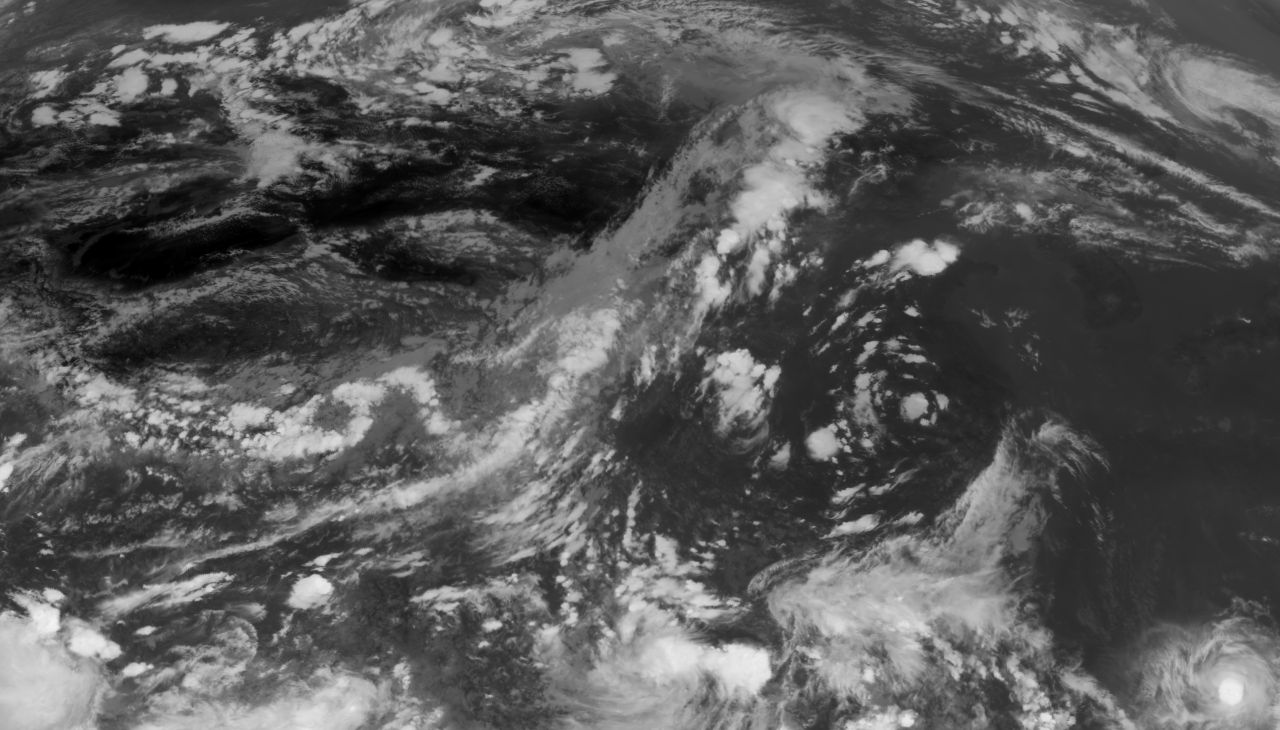
\includegraphics[width=\linewidth]{0001 (1).png}}
	\end{minipage}&
	\begin{minipage}[b]{0.15\columnwidth}
		\centering
		\raisebox{-.5\height}{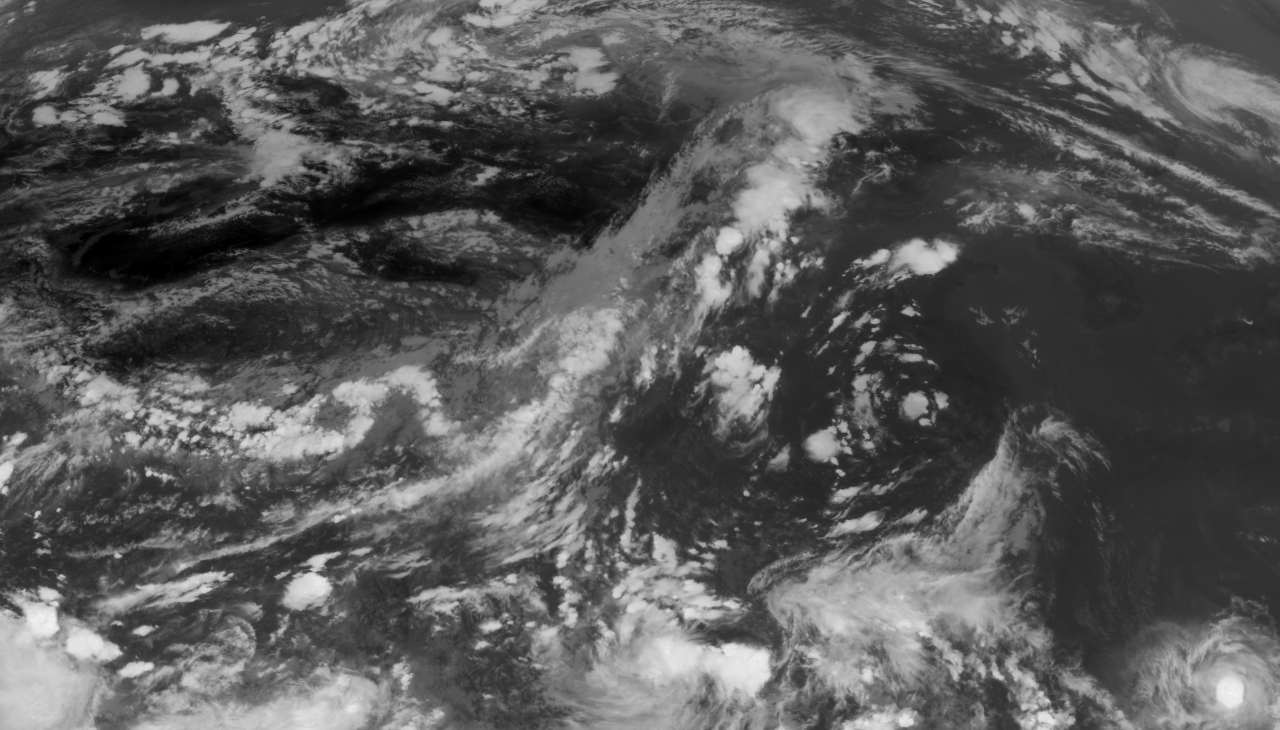
\includegraphics[width=\linewidth]{0001 (2).png}}
	\end{minipage}& 
	\begin{minipage}[b]{0.15\columnwidth}
		\centering
		\raisebox{-.5\height}{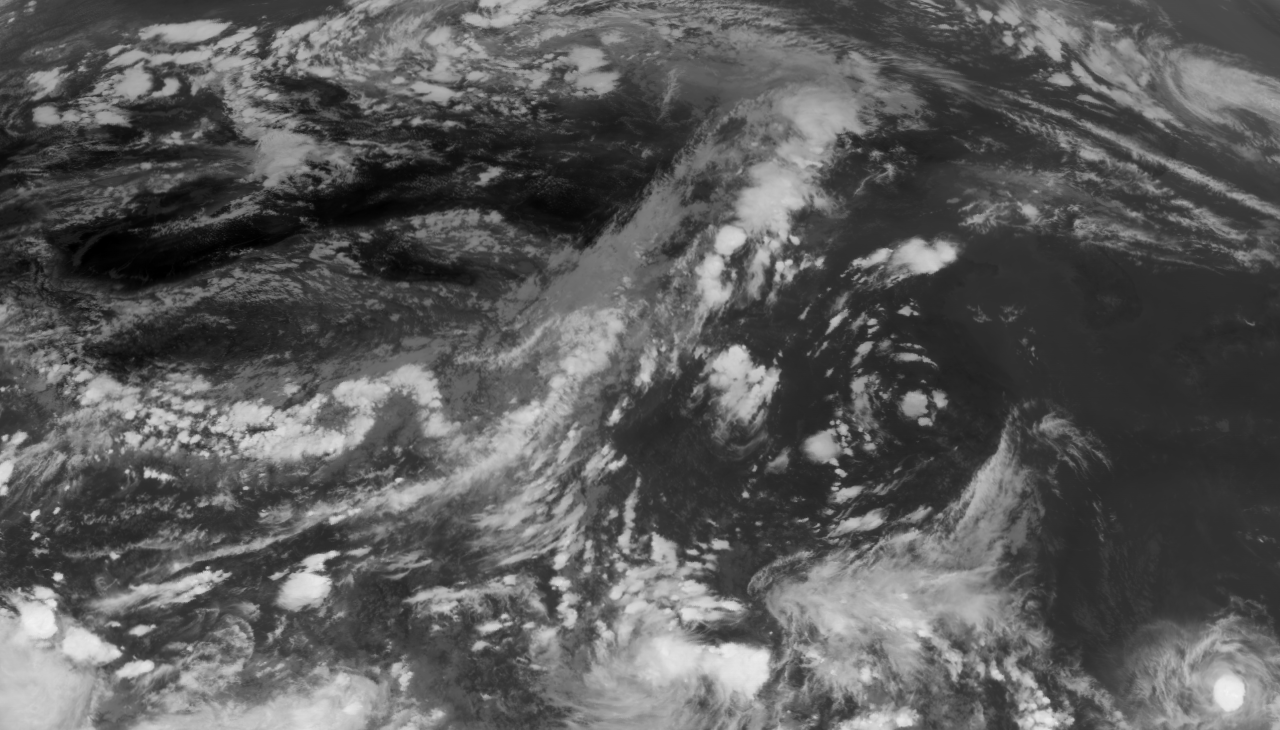
\includegraphics[width=\linewidth]{0001 (3).png}}
	\end{minipage}\\
	\\
			红外通道IR2 &
	\begin{minipage}[b]{0.15\columnwidth}
		\centering
		\raisebox{-.5\height}{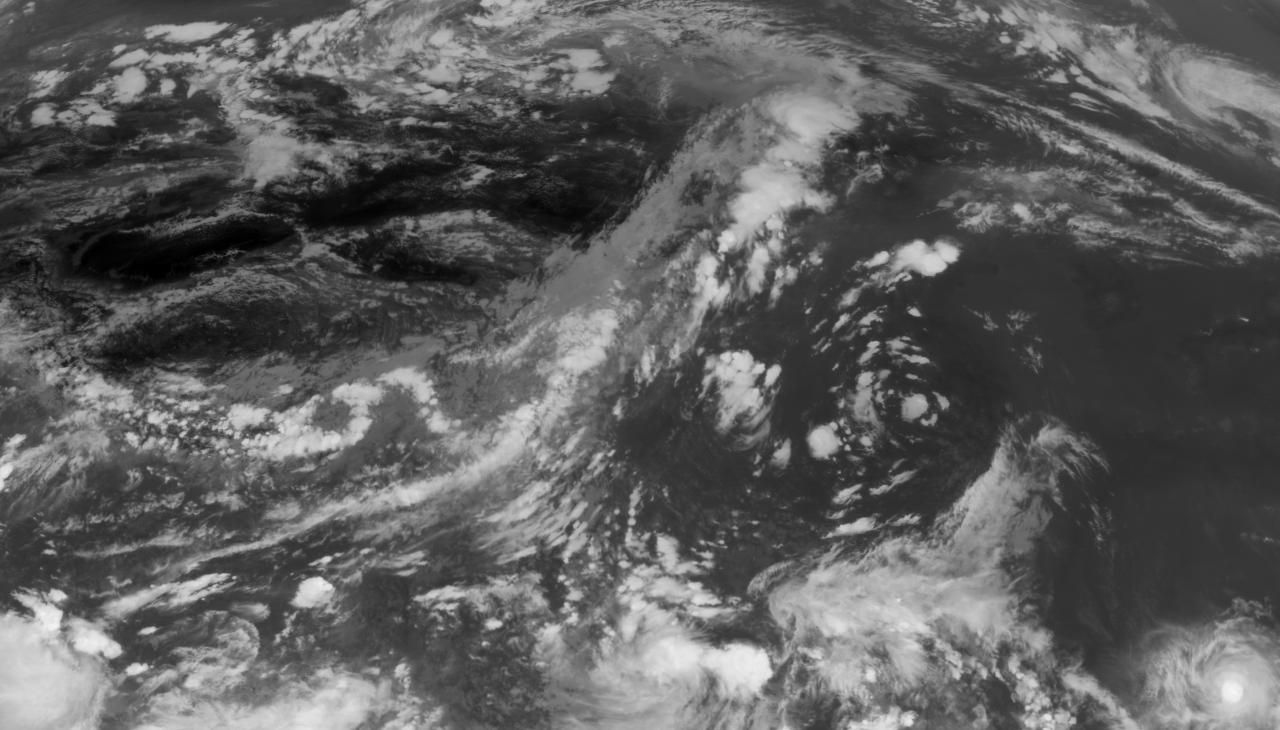
\includegraphics[width=\linewidth]{0002.png}}
	\end{minipage}&
	\begin{minipage}[b]{0.15\columnwidth}
		\centering
		\raisebox{-.5\height}{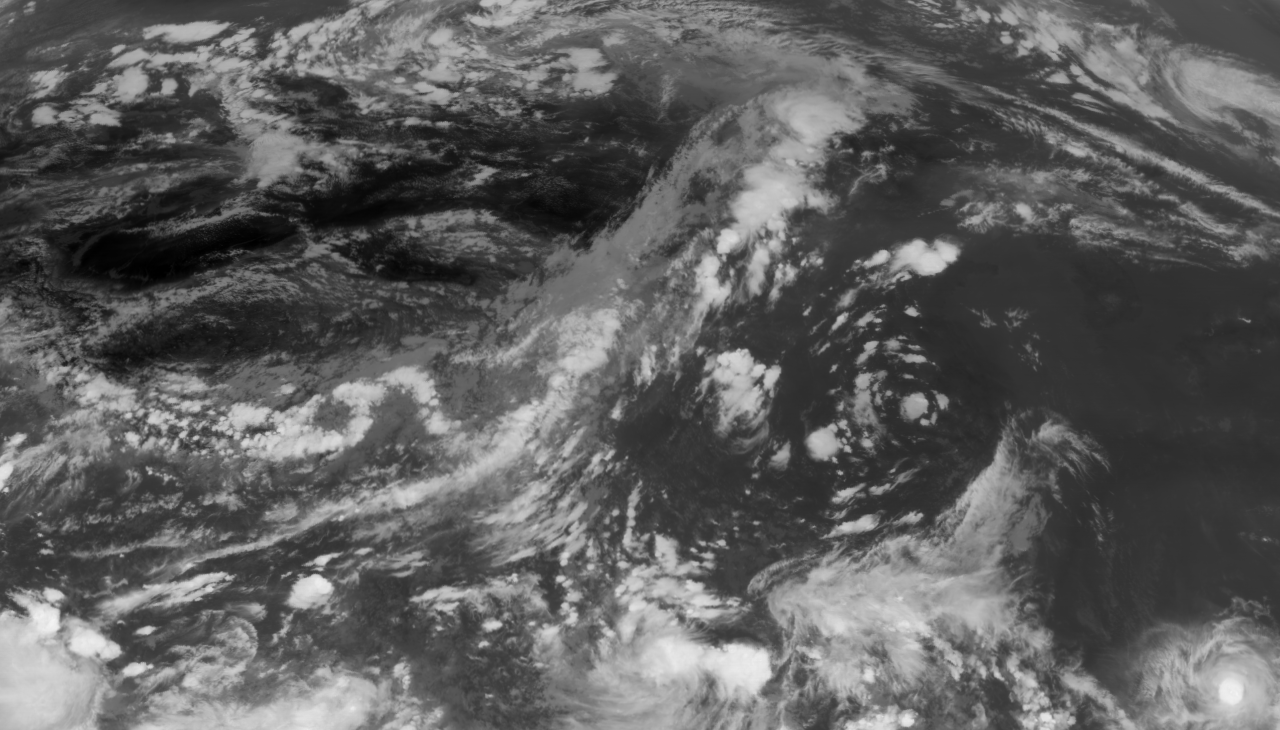
\includegraphics[width=\linewidth]{0002 (1).png}}
	\end{minipage}&
	\begin{minipage}[b]{0.15\columnwidth}
		\centering
		\raisebox{-.5\height}{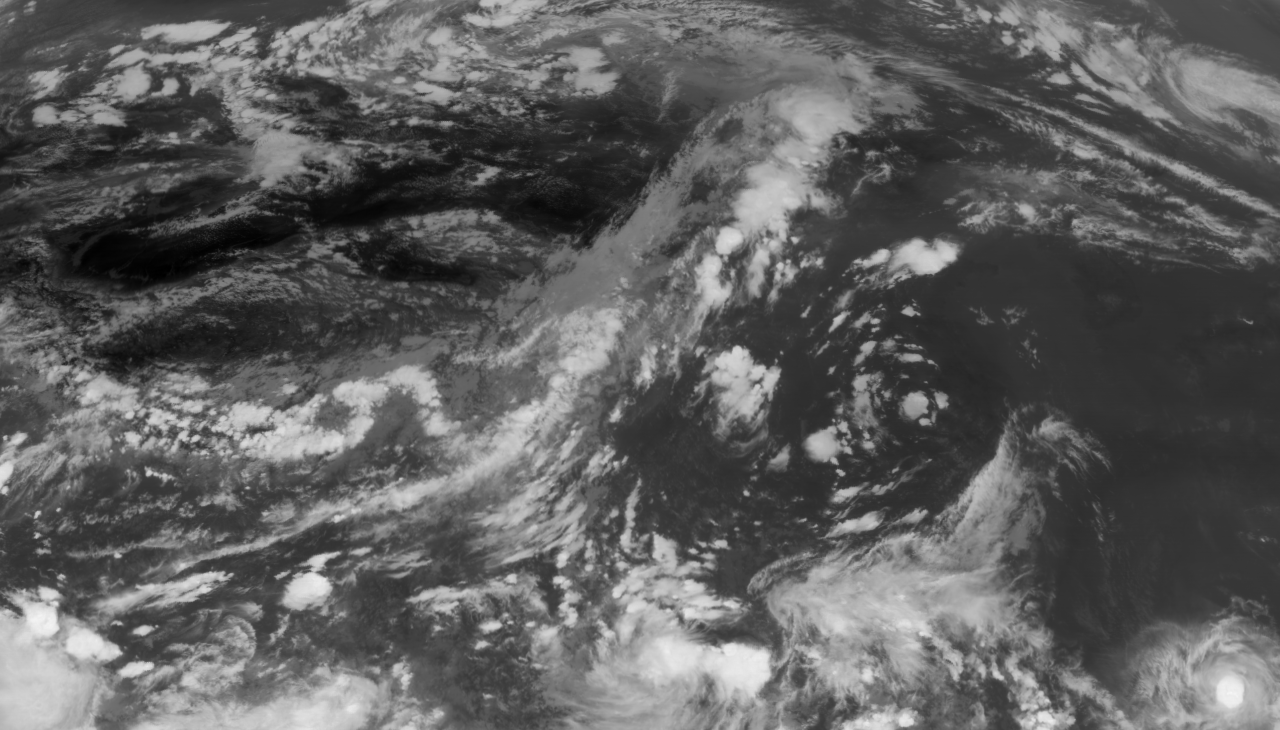
\includegraphics[width=\linewidth]{0002 (2).png}}
	\end{minipage}& 
	\begin{minipage}[b]{0.15\columnwidth}
		\centering
		\raisebox{-.5\height}{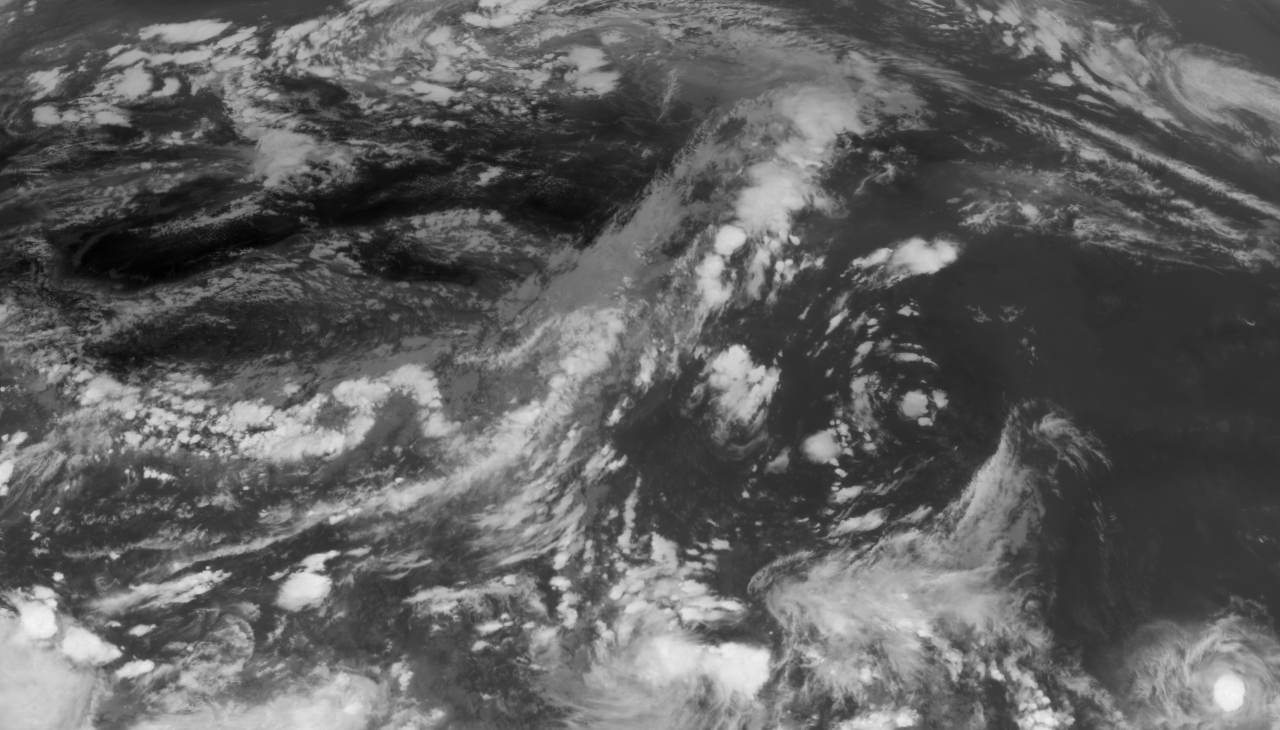
\includegraphics[width=\linewidth]{0002 (3).png}}
	\end{minipage}\\
	\\
 \hline
	\end{tabular}
\end{table}
\begin{table}[h]
	\centering
	\label{tb_vis_dataset_label}
	\caption{初生对流可视化类别标注即掩码展示图}
	\begin{tabular}{c c}
		\hline 可视化类别标注结果 & 类别标注掩码 \\
		\hline \\
		\begin{minipage}[b]{0.42\columnwidth}
			\centering
			\raisebox{-.5\height}{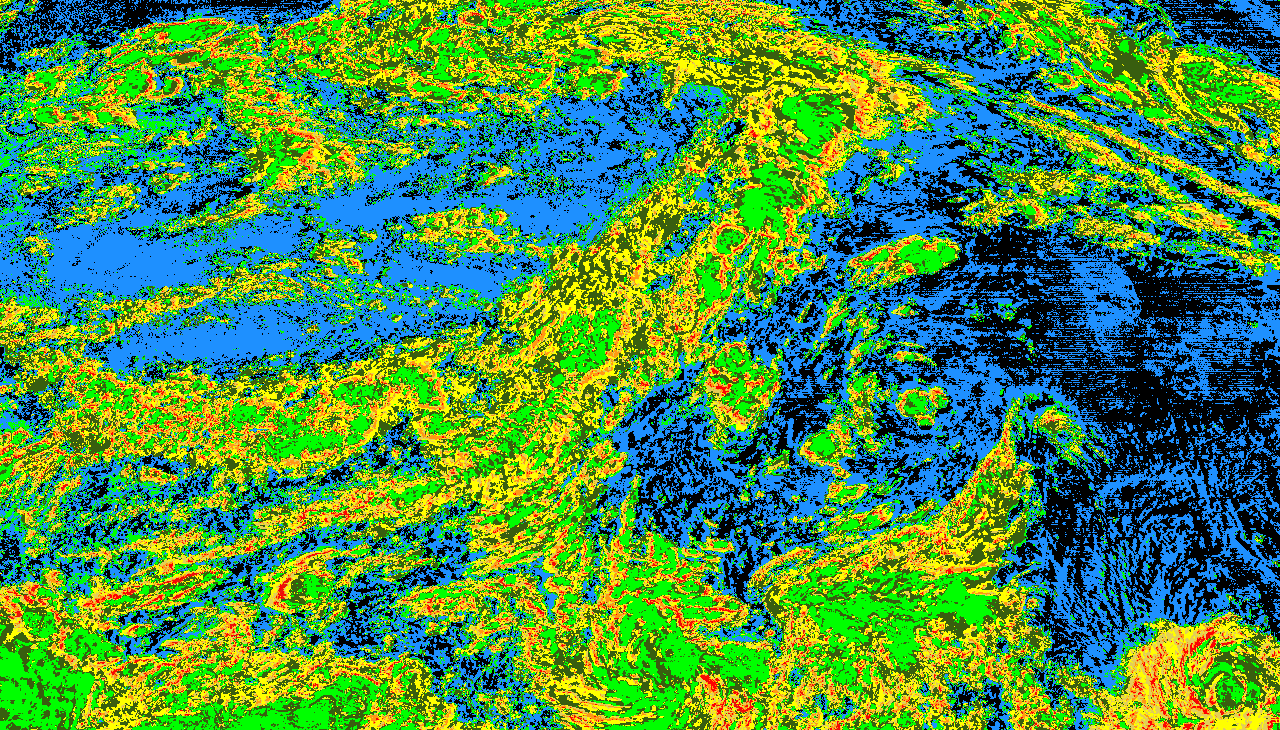
\includegraphics[width=\linewidth]{000mp.png}}
		\end{minipage}&
		\begin{minipage}[b]{0.42\columnwidth}
			\centering
			\raisebox{-.5\height}{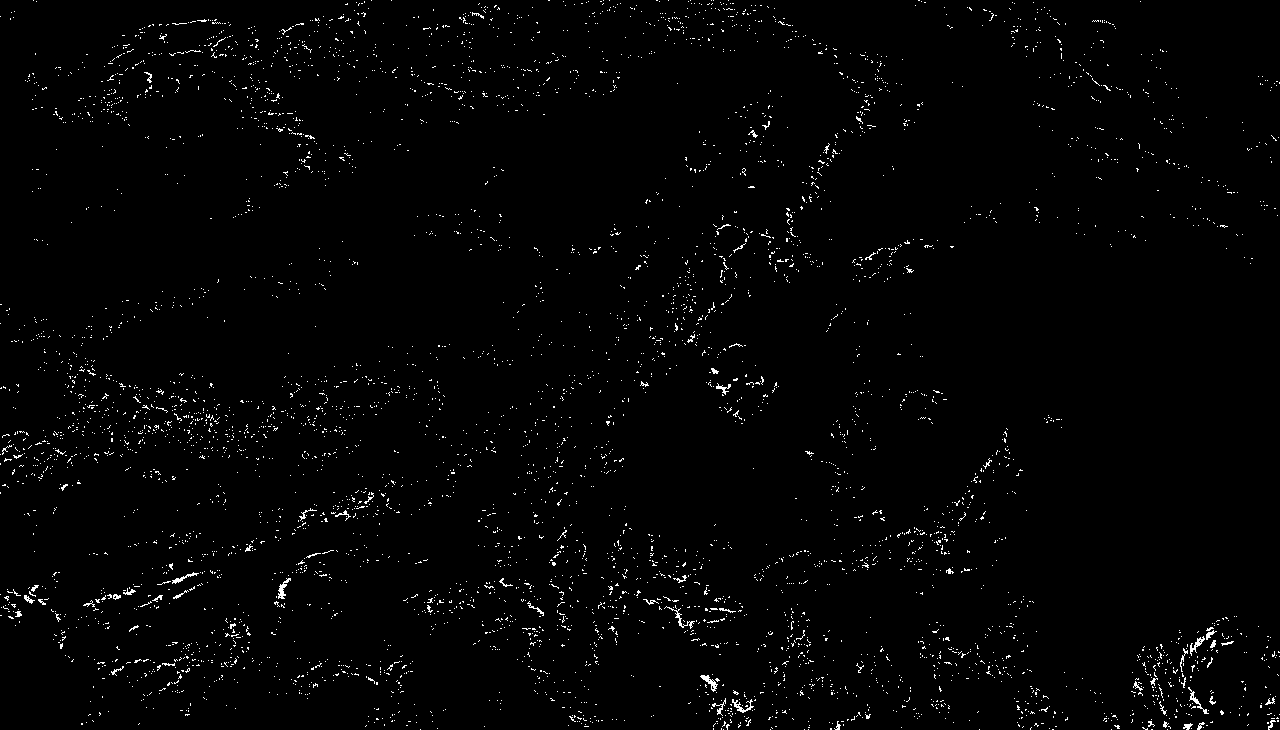
\includegraphics[width=\linewidth]{000lb.png}}
		\end{minipage} \\
	\\
	\hline
	\end{tabular}
\end{table}

经过统计分析,每张类别标注图像中存在初生对流的平均比率为0.79\%,平均每张图像存在7457个初生对流样本像元。可见其中的类别比例严重失衡。

\subsection{融合DenseConnection的RCNN模型结构}

对于像素级分类这一问题,本课题采用了RCNN模型作为基础模型进行初生对流的预测工作。初生对流多存在于云团系的边缘附近,因此要判识初生对流,模型至少需要一个像元附近的周围的像元来判别是否在云团边缘,从而更好的判识初生对流。一般初生对流所联通的区域很小,通常仅仅是一个或者几个像元相联通,而其中一个像元单独存在且不连通的样本占绝大多数。因此本课题所采用的模型是能够擅长处理像素级分类的循环卷积神经网络RCNN。

RCNN模型是逐步缩小检测范围的多层卷积神经网络结构,相比CNN能够复用不同尺度特征,有效提取像元的空间信息。RCNN模型相比于语义分割模型(Unet、Deeplab)等对于处理单个像元分类的任务要更加优秀,语义分割模型更擅长处理大范围联通样本分类问题。

基础的RCNN模型如图~\ref{RCNN_model}~所示:

\begin{figure}[h]
	\centering
	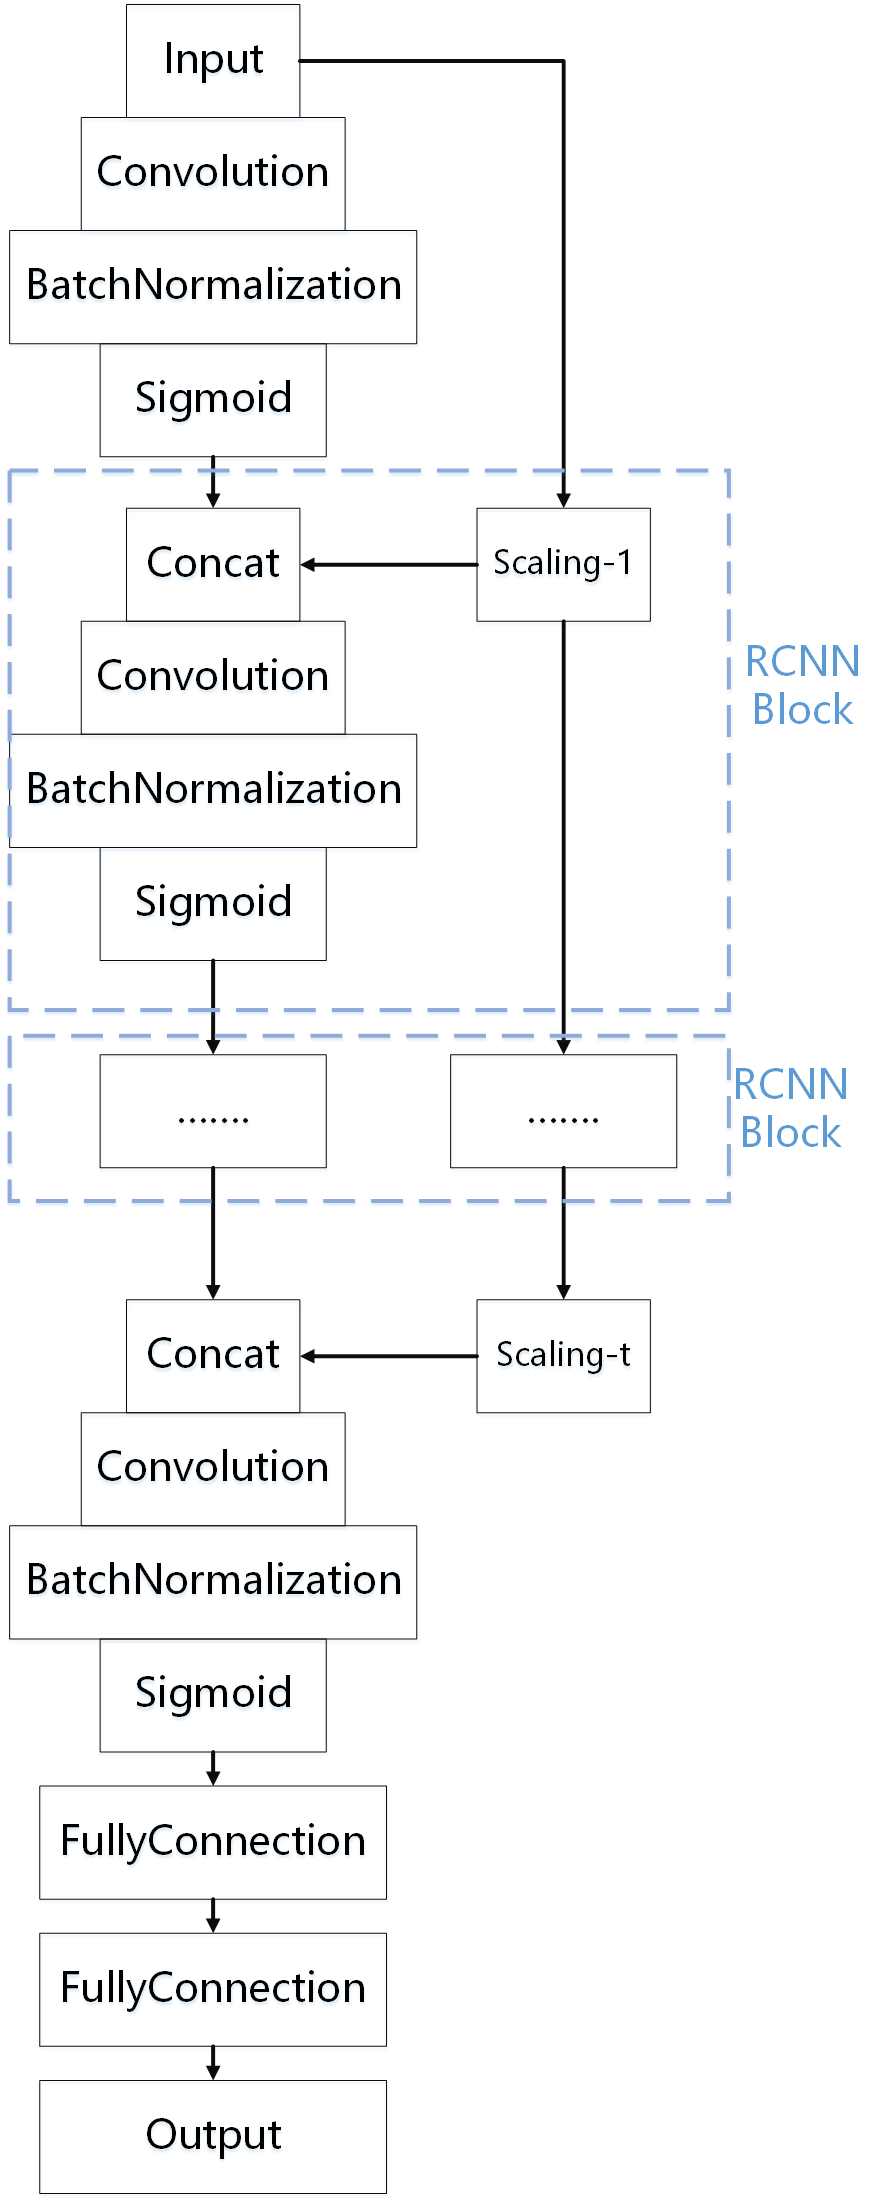
\includegraphics[width = 0.4\textwidth]{RCNN模型框架.png}
	\caption{RCNN模型框架}
	\label{RCNN_model}
\end{figure}

RCNN模型中基本的结构为RCNN Block,由一次2D卷积一次批标准化以及一层激活函数组成。RCNN Block每层所接受的输入为上一层的结果以及原始图像缩放后经过通道连接的张量。由~\ref{feature_importance}~,可见其中对于越靠近像元中心的像元,其RCNN的模型对其的附加的权重就越大。

\begin{figure}[h]
	\centering
	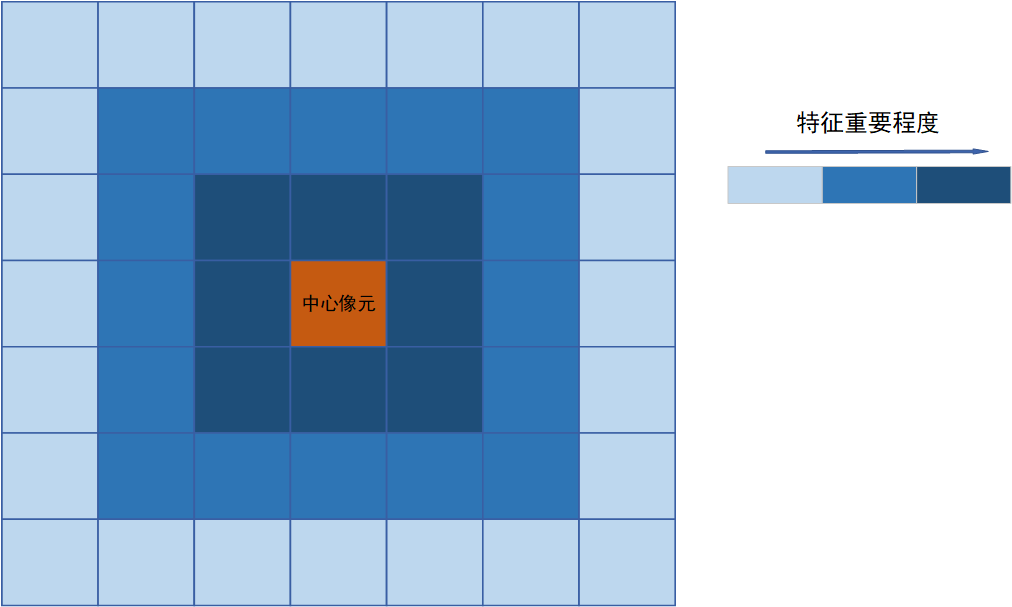
\includegraphics[width = 0.4\textwidth]{特征重要程度.png}
	\caption{特征重要程度}
	\label{feature_importance}
\end{figure}

然而真实情况下单独依靠像元中心并不能判识初生对流,甚至无法判识云团边缘。不同层级的RCNN卷积核用于提取不同尺度的特征,随着层数加深卷积核所提取的特征所概况的空间信息越少,而很多情况下初生对流所依赖的特征所属于较初始的低阶特征,因此这里引入DenseConnection结构,每次卷积都保留上一层所有的特征图,对特征依次传递保留,如~\ref{Dense_RCNN_model}~所示。

\begin{figure}[h]
	\centering
	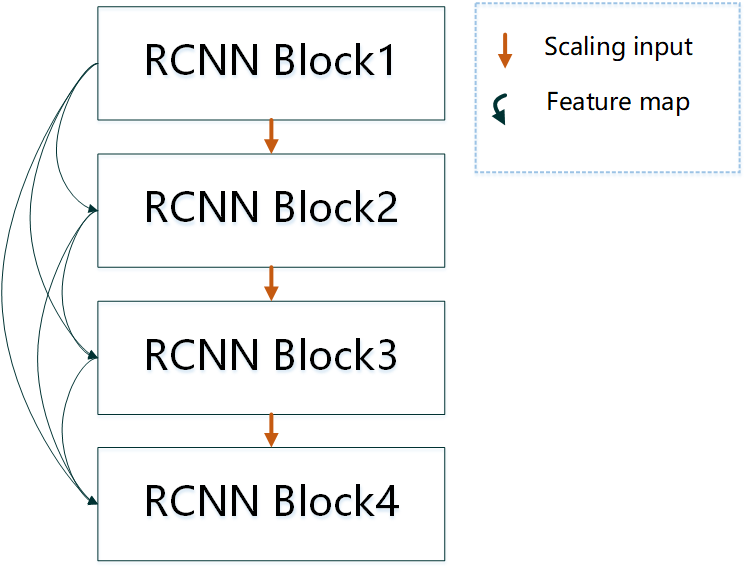
\includegraphics[width = 0.4\textwidth]{block.png}
	\caption{Dense-RCNN连接结构}
	\label{Dense_RCNN_model}
\end{figure}

Dense-RCNN相较于RCNN精度有较为明显的提升,DenseConnection来源于DenseNet,DenseNet的后序之作SENet是基于DenseNet在深度卷积神经网络中的数据集中取得了更好的效果。SE结构在DenseConnection上加以改进,上一层特征通道的简单叠加替换为了附加权重的特征叠加,通过一层特征选择支流给特征赋予权重。SE-RCNN相比Dense-RCNN结果的精度又有微弱提升。

\begin{figure}[h]
	\centering
	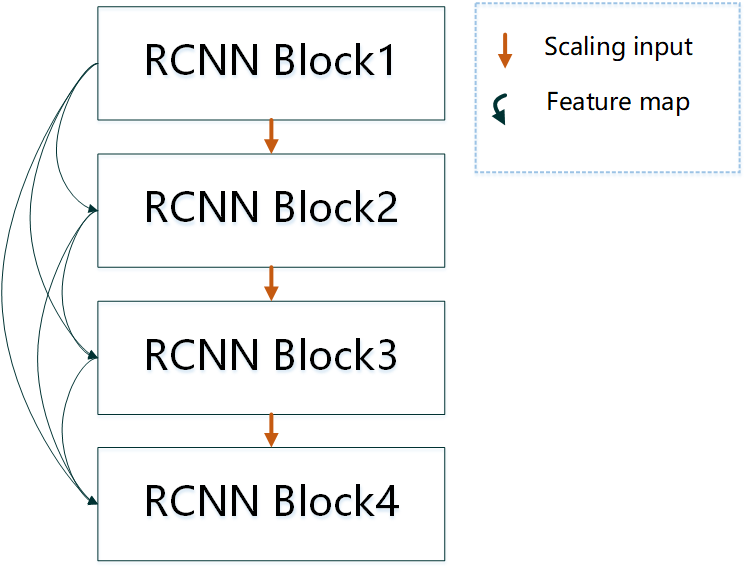
\includegraphics[width = 0.4\textwidth]{block.png}
	\caption{Dense-RCNN连接结构}
	\label{Dense_RCNN_model}
\end{figure}
